% !TeX program = lualatex

% Author: Malte, DE7LMS
% Year: 2022
% TH204 capacitor with label n47


\usepackage{siunitx}

\usepackage{amsmath}
\usepackage{unicode-math}
\setmathfont{Fira Math}
\setmathfont[range=up]{Roboto}
\setmathfont[range=it]{Roboto-Italic}
\setmathfont[range=\int]{Fira Math}
\usepackage[euler]{textgreek}
\usetikzlibrary{backgrounds}

\begin{document}

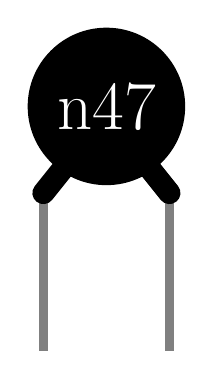
\begin{tikzpicture}[line cap=round]
  \fill (0,0) circle [radius=1cm];
  \draw[line width=8pt]
    (-.4,-.6) -- ++(-.4,-.5) coordinate (a)
    (.4,-.6) -- ++(.4,-.5) coordinate (b);
  \begin{pgfonlayer}{background}
    \draw[line width=3pt, gray]
      (a) -- ++(0,-2)
      (b) -- ++(0,-2);
  \end{pgfonlayer}
  \node[white,font=\Huge] at (0,0) {n47};
\end{tikzpicture}

\end{document}


